\documentclass{article}
\usepackage{graphicx}
\usepackage[T1]{fontenc}
\usepackage[utf8]{inputenc}
\usepackage{lmodern}
\usepackage{microtype}
\usepackage{tabularx}
\usepackage{array}
\newcolumntype{Y}{>{\raggedright\arraybackslash}X}
\usepackage{amsmath}
\usepackage{amssymb}
\usepackage{amsthm}
\usepackage{hyperref}
\usepackage{listings}
\usepackage{xcolor}
\usepackage[breakable,skins]{tcolorbox}
\tcbset{annotation/.style={enhanced,breakable,lines before break=4,boxrule=0pt,frame hidden,
  borderline west={1pt}{0pt}{gray!60},colback=gray!5,
  sharp corners,left=8pt,right=8pt,top=5pt,bottom=5pt,
  fontupper=\small,fonttitle=\small\bfseries,coltitle=black,
  attach title to upper={\par\smallskip},before skip=8pt,after skip=8pt}}
\newtcolorbox{implementationnote}{annotation,title=Implementation note}
\newtcolorbox{developmentnote}{annotation,title=Future development,
  colback=blue!3,borderline west={1pt}{0pt}{blue!45!black}}
\usepackage{booktabs}
\usepackage{geometry}
\usepackage{tikz}
\usepackage{tikz-cd}
\geometry{margin=1in}
\hypersetup{hidelinks, pdftitle={The Mathematics of tagd}, pdfauthor={Isaac N Colley}}
\setlength{\emergencystretch}{2em}

% Theorem environments
\newtheorem{definition}{Definition}[section]
\newtheorem{theorem}{Theorem}[section]
\newtheorem{proposition}{Proposition}[section]
\newtheorem{corollary}{Corollary}[section]
\newtheorem{remark}{Remark}[section]

% Code listing style for TAGL
\lstdefinelanguage{TAGL}{
  keywords={},
  sensitive=false,
  comment=[l]{--},
  morecomment=[s]{-*}{*-},
  morestring=[b]",
}
\lstdefinestyle{tagl}{
  language=TAGL,
  basicstyle=\ttfamily\small,
  keywordstyle=\color{blue},
  commentstyle=\color{gray}\itshape,
  stringstyle=\color{teal},
  backgroundcolor=\color{gray!8},
  frame=single,
  framesep=4pt,
  rulecolor=\color{gray!40},
  breaklines=true,
  captionpos=b,
}

% Code listing style for C++
\lstdefinestyle{cpp}{
  language=C++,
  basicstyle=\ttfamily\small,
  keywordstyle=\color{blue},
  commentstyle=\color{gray}\itshape,
  stringstyle=\color{teal},
  backgroundcolor=\color{gray!8},
  frame=single,
  framesep=4pt,
  rulecolor=\color{gray!40},
  breaklines=true,
  captionpos=b,
}

\title{\textbf{The Mathematics of tagd}\\
\large A Formal Description of the Mathematical Structures\\
in the tagd Semantic-Relational System}
\author{Isaac N Colley}
\date{September 2026}

\begin{document}
\pdfbookmark[1]{Title Page}{title}

\maketitle

\begin{center}
    \textit{``To be, is to be related.''} \\[0.5ex]
    \small --- tagd Maxim
\end{center}

\begin{abstract}
The tagd system was built from engineering instincts about how knowledge should
be structured. This paper makes the mathematics of those instincts explicit.
Its central thesis is that \emph{information is structural}: in tagd, meaning
is defined through relations. A tag is situated by its subordinate relation
and described by its predicates. Rank strings encode this hierarchy as a
partial order, whose Alexandrov topology gives precise form to containment,
neighbourhoods, and continuity. The paper develops these connections and
explores how they can support a relational account of computation.
\end{abstract}

\tableofcontents
\bigskip

\section{Primitives}

\subsection{Tags}

A \textbf{tag} is the atomic unit of the tagd system: a node in the
hierarchy and a point in the tagspace topology developed below. Tag
identifiers are UTF-8 labels \cite{readme}. A tag carries two distinct identities:

\begin{itemize}
  \item \textbf{Nominal identity}: a UTF-8 label unique within a tagspace.
  \item \textbf{Structural identity}: its position in the tagspace hierarchy,
        given by its rank, defined by its subordinate relation (aka identity
        relation) \cite{spec}.
\end{itemize}

\begin{definition}[Tag Set]
Let $T$ be the set of all tags in a tagspace. Each tag $t \in T$ is identified
by a string $\mathrm{id}(t) \in \Sigma^*$, where $\Sigma^*$ denotes the set of
all finite UTF-8 strings.
\end{definition}

In TAGL, defining a tag looks like:
\begin{lstlisting}[style=tagl, caption={Defining a tag via a subordinate relation}]
>> dog _is_a mammal;
\end{lstlisting}
Here \texttt{dog} is a tag. Its nominal identity is the string \texttt{"dog"}.
Its structural identity is defined by its subordinate relation to
\texttt{mammal}.

\subsection{The Root and the Axiom}

Every tagspace has a distinguished root tag: \texttt{\_entity}. The README
states:
\begin{quote}
\texttt{\_entity} is axiomatic and self-referencing
(i.e.\ \texttt{\_entity \_sub \_entity}). It is the only tag having this
relation. It is the root of a tagspace.
\end{quote}

\begin{definition}[Axiomatic Root]
The tag \texttt{\_entity} is the \textbf{axiomatic root} of every tagspace. It
is the unique fixed point of the parent function extended to the root: the one tag whose
super-object is itself.
\end{definition}

In TAGL notation:
\begin{lstlisting}[style=tagl, caption={The axiomatic root}]
_entity _sub _entity
\end{lstlisting}

The symbolic operator \texttt{<:} maps to \texttt{\_sub} exactly.
\begin{lstlisting}[style=tagl, caption={TAGL subordinate symbol}]
_entity <: _entity
\end{lstlisting}

In hierarchical terms, \texttt{\_entity} is the \textbf{root} of the tagspace
--- the tag that is an ancestor of everything, including itself.

\section{The Subordinate Relation and the Rooted Tree}

\subsection{Subordinate Relations}

A tag's structural identity is defined by one subordinate (sub) relation:
a sub-relator and a parent \cite{spec,thesis}. The code represents these as
\texttt{sub\_relator} and \texttt{super\_object}.

The sub relators are defined in \texttt{hard-tags.h} \cite{hardtags}:
\begin{lstlisting}[style=cpp, caption={Sub relator definitions in hard-tags.h}]
inline constexpr std::string_view HARD_TAG_SUB{"_sub"}; /// HARD_TAG_SUB HARD_TAG_ENTITY tagd::POS_SUB_RELATOR
// Leibniz discernment from _sub will come as constraints in TAGL are developed
inline constexpr std::string_view HARD_TAG_IS_A{"_is_a"}; /// HARD_TAG_SUB HARD_TAG_SUB tagd::POS_SUB_RELATOR
inline constexpr std::string_view HARD_TAG_TYPE_OF{"_type_of"}; /// HARD_TAG_SUB HARD_TAG_SUB tagd::POS_SUB_RELATOR
\end{lstlisting}

A typical TAGL knowledge hierarchy:
\begin{lstlisting}[style=tagl, caption={Building a subordinate hierarchy in TAGL}]
>> physical_object _sub _entity;
>> living_thing _type_of physical_object;
>> animal _type_of living_thing;
>> mammal _type_of animal;
>> dog _is_a mammal;
\end{lstlisting}

\begin{remark}[Direct subordination versus containment]
A subordinate relation records the pair $(s,p(t))$, where $s$ is its
sub-relator and $p(t)$ its immediate parent. This edge is distinct from the
reflexive, transitive ancestor relation encoded by rank prefixes. For a
non-root tag, the parent is its unique lower cover in the ancestor-first
order used below; the root has no lower cover.
\end{remark}

\subsection{The Tagspace as a Rooted Tree}

The subordinate relation organizes tags into a \textbf{rooted tree}.

\begin{definition}[Tagspace Tree]
A tagspace is a pair $(T, p)$ where:
\begin{itemize}
  \item $T$ is a set of tags containing the distinguished root
        \texttt{\_entity},
  \item $p : T \setminus \{\texttt{\_entity}\} \to T$ is the \emph{parent
        function}, assigning each non-root tag its super-object.
\end{itemize}
Every non-root tag reaches \texttt{\_entity} after finitely many parent
steps. There are no cycles (except the axiomatic self-reference of
\texttt{\_entity}, when $p$ is extended to the root).
\end{definition}

The tree structure of the example above:
\begin{verbatim}
_entity
  physical_object
    living_thing
      animal
        mammal
          dog
\end{verbatim}

The tree expresses hierarchical knowledge: \texttt{dog} is related to
\texttt{mammal}, which is related to \texttt{animal}, and so on. Each
parent step contributes to the tag's structural identity.

\begin{developmentnote}
Here \texttt{\_is\_a} and \texttt{\_type\_of} both establish subordination;
their finer logical interpretation is discussed in Section~\ref{sec:future}.
\end{developmentnote}

\section{Rank: Encoding the Tree in Strings}

\subsection{The Rank Function}

Each tag is assigned a \textbf{rank} --- a UTF-8 byte string encoding its
position in the tagspace tree. The \texttt{rank.h} source states:
\begin{quote}
A rank string is the ordinal value of each node in the tagspace tree. A code
point at a particular level is known as the rank value.
\end{quote}

\begin{definition}[Rank Function]
The rank function $r : T \to \Sigma^*$ assigns to each tag a UTF-8 string
such that $r$ is injective and a child's rank extends its parent's rank by
one code point. The root has the empty rank.
\end{definition}

For example, the following hard tags have these ranks. Dots separate the
code points along a path; the stored rank is a byte string \cite{bootstrap}:

\begin{center}
\begin{tabularx}{\textwidth}{@{}YYY@{}}
\toprule
\textbf{Tag} & \textbf{Rank (dotted)} & \textbf{Position} \\
\midrule
\texttt{\_entity}       & (empty)  & level 0, root \\
\texttt{\_sub}          & 1        & level 1 \\
\texttt{\_is\_a}        & 1.1      & level 2 \\
\texttt{\_type\_of}     & 1.2      & level 2 \\
\texttt{\_rel}          & 2        & level 1 \\
\texttt{\_has}          & 2.1      & level 2 \\
\texttt{\_true}         & 3        & level 1 \\
\texttt{\_false}        & 4        & level 1 \\
\texttt{\_interrogator} & 5        & level 1 \\
\bottomrule
\end{tabularx}
\end{center}

\subsection{The Prefix Partial Order}

The key property of ranks is stated explicitly in \texttt{rank.h}:
\begin{quote}
All children of a particular node in the rank hierarchy will be prefixed by the
parent node --- that is, rank substrings define subtrees in the hierarchy.
\end{quote}

\begin{definition}[Containership Relation]
Define the \textbf{containership relation} $\sqsubseteq$ on $T$ by:
\[
  a \sqsubseteq b
  \iff
  r(a) \text{ is a prefix of } r(b).
\]
That is, $a \sqsubseteq b$ means $a$ is an ancestor of $b$ (or $a = b$). Tag
$a$ \emph{contains} tag $b$ in the hierarchy.
\end{definition}

For nonempty ranks, this prefix test is declared in \texttt{rank.h} and
implemented by \texttt{rank::contains()} in \texttt{rank.cc}:
\begin{lstlisting}[style=cpp, caption={Containership via rank prefix in rank.h}]
// this rank contains the rank being compared,
// in other words, this rank is a prefix to the other
bool contains(const rank&) const;
\end{lstlisting}

\begin{implementationnote}
The root is represented by the empty prefix. The tagspace-level containment
API handles it explicitly; \texttt{rank::contains()} compares nonempty ranks.
\end{implementationnote}

The nonempty-rank test is used in \texttt{tagd.cc} for structural operations on tag sets:
\begin{lstlisting}[style=cpp, caption={Containership used in merge\_containing\_tags (tagd.cc)}]
if (b->rank().contains(a->rank())) { // rank can contain itself (b == a)
    merged++;
} else if (a->rank().contains(b->rank())) {
    A.insert(*b);
}
\end{lstlisting}

\subsection{Verifying the Partial Order Axioms}

\begin{theorem}
The containership relation $\sqsubseteq$ is a partial order on $T$.
\end{theorem}

\begin{proof}
We verify the three required properties.

\textbf{Reflexivity.} Every string, including the empty string, is a prefix
of itself. Hence $a \sqsubseteq a$ for all $a \in T$.

\textbf{Antisymmetry.} Suppose $a \sqsubseteq b$ and $b \sqsubseteq a$. Then
$r(a)$ is a prefix of $r(b)$ and $r(b)$ is a prefix of $r(a)$. A string $u$
is a prefix of $v$ and $v$ is a prefix of $u$ if and only if $u = v$. Hence
$r(a) = r(b)$, which implies $a = b$ since ranks uniquely identify a tag's
position in a tagspace.

\textbf{Transitivity.} Suppose $a \sqsubseteq b$ and $b \sqsubseteq c$. Then
$r(a)$ is a prefix of $r(b)$ and $r(b)$ is a prefix of $r(c)$. Since the
prefix relation on strings is transitive, $r(a)$ is a prefix of $r(c)$, so
$a \sqsubseteq c$.
\end{proof}

Therefore $(T, \sqsubseteq)$ is a \textbf{poset} (partially ordered set).

\subsection{Subtrees and Their Intersection}

For $x\in T$, define the descendant subtree, including its root, by
\[
 D(x)=\{t\in T:x\sqsubseteq t\}.
\]
The unique-parent property makes this family \emph{laminar}: two subtrees
are nested or disjoint. Explicitly,
\[
D(x)\cap D(y)=
\begin{cases}
D(y),&x\sqsubseteq y,\\
D(x),&y\sqsubseteq x,\\
\varnothing,&\text{otherwise}.
\end{cases}
\]
If a tag belonged to both subtrees, both roots would lie on its unique
ancestor chain and hence would be comparable. This proves the last case;
the first two follow directly from transitivity.

For example, with \texttt{dog} and \texttt{cat} subordinate to \texttt{mammal},
and \texttt{bird} on a separate branch subordinate to \texttt{animal},
$D(\texttt{animal})\cap D(\texttt{mammal})=D(\texttt{mammal})$, whereas
$D(\texttt{mammal})\cap D(\texttt{bird})=\varnothing$.
This is the set-theoretic basis for retaining the more specific root when
intersecting subtree selections. A descendant subtree does not include its
root's strict ancestors; shared ancestry therefore does not change the
empty-intersection case. Common ground between entire tagspaces is
considered in Section~\ref{sec:common-ground}.

\begin{center}
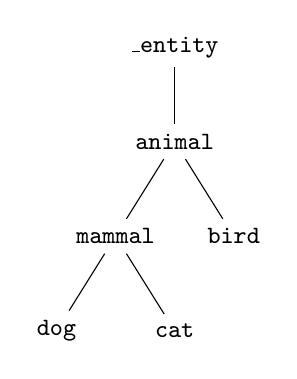
\begin{tikzpicture}[level distance=1.2cm,
  level 1/.style={sibling distance=3cm},
  level 2/.style={sibling distance=1.5cm},
  every node/.style={font=\ttfamily\small}]
  \node {\_entity}
    child {node {animal}
      child {node {mammal}
        child {node {dog}}
        child {node {cat}}
      }
      child {node {bird}}
    };
\end{tikzpicture}
\end{center}

\subsection{Lexicographic Total Order}

Ranks also carry a total \textbf{lexicographic order}, implemented in
\texttt{rank.h}:
\begin{lstlisting}[style=cpp, caption={Lexicographic ordering of ranks}]
bool operator<(const rank& rhs) const { return _data < rhs._data; }
\end{lstlisting}

This order --- a deliberate UTF-8 design choice noted in \texttt{rank.h}
(``it collates lexicographically'') --- enables efficient storage and retrieval
of ranks as a sorted structure. Tags within the same subtree sort together.
The hierarchy is therefore encoded directly in the ordering of the index.

\begin{implementationnote}
SQLite uses \texttt{COLLATE BINARY} for the rank column and
\texttt{ORDER BY rank} in \texttt{.dump\_grid} \cite{sqlite}.
\end{implementationnote}

\subsection{CS Tree versus Topological Poset: Orientation}

A tree drawing places \texttt{\_entity} at the top, but the ancestor-first
prefix order makes it the \textbf{least element} ($\bot$): its empty rank
prefixes every rank and has the lowest value under binary lexicographic
collation using C++'s less-than operator \texttt{<}. This total order extends
the prefix partial order; it also compares unrelated branches. Leaves are
\textbf{maximal elements} of the partial order, not necessarily greatest in
lexicographic order.

\section{The Tagspace Topology}

\subsection{From Partial Order to Topology}

We choose the upper-set Alexandrov topology of the ancestor-first poset
$(T, \sqsubseteq)$ \cite{alexandrov}. This makes the tagspace a
topological space whose basic open sets are its subtrees:

\begin{definition}[Tagspace Open Sets]
A subset $U \subseteq T$ is \textbf{open} if it is upward-closed under
$\sqsubseteq$:
\[
  U \in \mathcal{T}
  \iff
  \forall\, a \in U,\; \forall\, b \in T :\;
  a \sqsubseteq b \Rightarrow b \in U.
\]
\end{definition}

In the tagspace tree, ``upward-closed'' means: if a tag is in the set, all
its descendants are too. The smallest open neighbourhood of $x$ is its subtree
\[
 N(x)=\{b\in T:x\sqsubseteq b\}=D(x)=\uparrow\!x.
\]
Each $D(x)$ is a principal filter; the closure of $\{x\}$ is its ancestry,
the principal ideal $\downarrow\!x=\{b\in T:b\sqsubseteq x\}$.
There is also a dual Alexandrov topology of downward-closed sets, in which
$D(x)$ is a closed set. Both topologies arise from the same tree; this
paper keeps the upward-open convention unless explicitly stated otherwise.

This construction is known as the \textbf{Alexandrov topology} --- the topology
generated by a partial order in which arbitrary intersections (not just finite
ones) of open sets remain open.

\subsection{Verifying the Topology Axioms}

\begin{theorem}
Let $T$ be the set of tags in a tagspace and let $\mathcal{T}$ be the
collection of upward-closed subsets under $\sqsubseteq$. Then
$(T, \mathcal{T})$ is a topological space.
\end{theorem}

\begin{proof}
We verify the three axioms.

\textbf{(i) $\emptyset \in \mathcal{T}$ and $T \in \mathcal{T}$.}
The empty set is vacuously upward-closed. The full set $T$ is upward-closed
because there is no $b \in T$ outside $T$. Both belong to $\mathcal{T}$.

\textbf{(ii) Finite intersections.}
Let $U, V \in \mathcal{T}$. Suppose $a \in U \cap V$ and $a \sqsubseteq b$.
Then $b \in U$ (since $U$ is upward-closed) and $b \in V$ (since $V$ is
upward-closed), so $b \in U \cap V$. Hence $U \cap V \in \mathcal{T}$.

\textbf{(iii) Arbitrary unions.}
Let $\{U_\alpha\}$ be any collection of sets in $\mathcal{T}$. Suppose
$a \in \bigcup_\alpha U_\alpha$ and $a \sqsubseteq b$. Then $a \in U_\alpha$
for some $\alpha$. Since $U_\alpha$ is upward-closed, $b \in U_\alpha
\subseteq \bigcup_\alpha U_\alpha$. Hence $\bigcup_\alpha U_\alpha \in
\mathcal{T}$.
\end{proof}

The intersection argument also holds for arbitrary families, establishing
the Alexandrov property. Therefore $(T, \mathcal{T})$ is a
\textbf{topological space}. The following excerpt from
\texttt{merge\_containing\_tags} illustrates the comparable-root cases of
subtree intersection: containment of their roots identifies which subtree
to retain. Representing subtrees by their roots connects the set-theoretic
operation to the rank-prefix test.
\begin{lstlisting}[style=cpp, caption={Intersection of subtrees in tagd.cc}]
if (b->rank().contains(a->rank())) {
    merged++;
} else if (a->rank().contains(b->rank())) {
    A.insert(*b);
}
\end{lstlisting}

\subsection{Specialization Order}

Every topological space carries a \textbf{specialization preorder}. We use
the convention $a\leq_{\mathrm{sp}}b$ if
$a\in\operatorname{cl}(\{b\})$.

\begin{proposition}
In the tagspace topology, $a\leq_{\mathrm{sp}}b$ if and only if
$a\sqsubseteq b$: the singleton closure consists of the tag and its ancestors.
\end{proposition}

Thus $\texttt{animal}\leq_{\mathrm{sp}}\texttt{mammal}
\leq_{\mathrm{sp}}\texttt{dog}$. Topological specialization in this
convention runs opposite to taxonomic specialization: the closure of a
specific tag contains its more general ancestors.

\subsection{Continuity as Order-Preservation}

\begin{definition}[Tagspace Map]
A map $f : T_1 \to T_2$ between two tagspaces is \textbf{topologically
continuous} if inverse images of open sets are open: $f^{-1}(U) \in \mathcal{T}_1$ for
every $U \in \mathcal{T}_2$.
\end{definition}

\begin{proposition}
A map $f : T_1 \to T_2$ is continuous (with respect to the Alexandrov
topologies) if and only if it is order-preserving: whenever
$a \sqsubseteq b$ in $T_1$, we have $f(a) \sqsubseteq f(b)$ in $T_2$.
\end{proposition}

This gives a precise mathematical definition of a
\textbf{hierarchy-preserving map} between tagspaces. If
\texttt{dog \_is\_a mammal} in $T_1$, a continuous map must send \texttt{dog}
to a descendant of the image of \texttt{mammal} in $T_2$, possibly that
image itself. Preserving labels, sub-relators, and predicates supplies
additional conditions when a map is to preserve the full semantic structure.

\section{The Hard Tag Base: A Common Subspace}

\subsection{Hard Tags}

Tagspaces initialized with the same hard-tag definitions contain
the same hard-tag hierarchy, defined in \texttt{hard-tags.h}
\cite{hardtags}:

\begin{lstlisting}[style=cpp, caption={Core hard tag definitions in hard-tags.h}]
inline constexpr std::string_view HARD_TAG_ENTITY{"_entity"}; /// HARD_TAG_SUB HARD_TAG_ENTITY tagd::POS_TAG
inline constexpr std::string_view HARD_TAG_SUB{"_sub"}; /// HARD_TAG_SUB HARD_TAG_ENTITY tagd::POS_SUB_RELATOR
inline constexpr std::string_view HARD_TAG_IS_A{"_is_a"}; /// HARD_TAG_SUB HARD_TAG_SUB tagd::POS_SUB_RELATOR
inline constexpr std::string_view HARD_TAG_TYPE_OF{"_type_of"}; /// HARD_TAG_SUB HARD_TAG_SUB tagd::POS_SUB_RELATOR
inline constexpr std::string_view HARD_TAG_RELATOR{"_rel"}; /// HARD_TAG_SUB HARD_TAG_ENTITY tagd::POS_RELATOR
inline constexpr std::string_view HARD_TAG_HAS{"_has"}; /// HARD_TAG_SUB HARD_TAG_RELATOR tagd::POS_RELATOR
inline constexpr std::string_view HARD_TAG_CAN{"_can"}; /// HARD_TAG_SUB HARD_TAG_RELATOR tagd::POS_RELATOR
inline constexpr std::string_view HARD_TAG_TRUE{"_true"}; /// HARD_TAG_SUB HARD_TAG_ENTITY tagd::POS_TRUE
inline constexpr std::string_view HARD_TAG_FALSE{"_false"}; /// HARD_TAG_SUB HARD_TAG_ENTITY tagd::POS_FALSE
inline constexpr std::string_view HARD_TAG_INTERROGATOR{"_interrogator"}; /// HARD_TAG_SUB HARD_TAG_ENTITY tagd::POS_INTERROGATOR
\end{lstlisting}

\subsection{The Hard Tag Subspace}

\begin{definition}[Hard Tag Subspace]
Let $H \subseteq T$ denote the set of hard tags. For tagspaces using the same
hard-tag definitions, the induced subspace topology on $H$ is the same,
since its restricted ancestry order is the same. Thus $H$ is a common
subspace shared by these tagspaces.
\end{definition}

\begin{remark}
One can define a category of extensions of $H$: objects are order embeddings
$i_T:H\hookrightarrow T$, and morphisms are monotone maps $f:T\to T'$
satisfying $f\circ i_T=i_{T'}$. In this category,
the object $H\xrightarrow{\mathrm{id}}H$ is \textbf{initial}: it has a unique
morphism to each object.
\end{remark}

\subsection{Interoperability via the Common Base}
\label{sec:common-ground}

Each tagspace is a world of discourse. When these worlds disagree about
user-defined tags, the same version of the hard-tag hierarchy $H$ supplies
common ground for exchanging and interpreting TAGL.

After identifying their copies of $H$, and any further tags whose identities
and structure agree, two tagspaces satisfy
\[
  H\subseteq T_1\cap T_2.
\]
If they share no user-defined tags, then $T_1\cap T_2=H$. Such tagspaces
need not be laminar: $T_1=H\cup\{a\}$ and $T_2=H\cup\{b\}$, with distinct
user tags $a,b$, overlap without either containing the other. Laminarity
applies to descendant subtrees within one tree. Equal labels alone do not
establish agreement between independently defined user tags.

\begin{developmentnote}
For extensions in which $H$ contains every ancestor of its tags, gluing
only the copies of $H$ gives a \textbf{categorical pushout}
$T_1\amalg_H T_2$ in posets with monotone maps. Keep the user tags distinct
and inherit each tree's parent relation. The result is again a rooted tree:
parents agree on $H$, and every other tag retains its original parent.
Any two monotone maps agreeing on $H$ extend uniquely to this union,
which is the pushout's universal property. The Alexandrov functor of
Section~8.1, being a left adjoint, carries this pushout to topological spaces.
This supplies a precise model for combining worlds; reconciling user labels,
predicates, and rank assignments remains part of the merge design.
\end{developmentnote}

\begin{implementationnote}
The hard-tag hierarchy provides the shared vocabulary used by \texttt{httagd},
the embedded HTTP application server having a Web API which maps to
\texttt{TAGL} - \emph{the language is the service}. Hard-tag definitions,
including ranks, can change between versions; the signed versioning scheme in
Section~\ref{sec:merkle} would make agreement on a particular base explicit.
\end{implementationnote}

\noindent\begin{minipage}{\linewidth}
\begin{lstlisting}[style=tagl, caption={A shared hard-tag version; distinct user extensions}]
-- shared by tagspaces using the same hard-tag version:
_entity _sub _entity

-- user-defined, varies by tagspace:
>> dog _is_a mammal;
\end{lstlisting}
\end{minipage}

\section{Predicates: Fibered Structure}

\subsection{Relators Are Tags}

Predicate relators are themselves tags --- subordinate to \texttt{\_rel} in
the tagspace tree. This means predicates are not outside the system; they are
\emph{inside} it. The tagspace is self-describing.

For example, predicate relators occupy related positions in the hierarchy
\cite{bootstrap}:
\begin{verbatim}
_rel     rank: 2        (root of predicate relators)
_has     rank: 2.1
_can     rank: 2.2
_refers  rank: 2.3
\end{verbatim}

The language used to attach meaning to tags is itself expressed in the same
structural language.

\subsection{Predicates as Horizontal Relations}

Predicates are relations attached to a tag that do not alter its position in
the tree. TAGL groups objects under a relator; each attached predicate
records one relator, one object, and optional modifier information
\cite{spec,tagdh}.

\begin{lstlisting}[style=tagl, caption={Vertical identity and horizontal predicates}]
>> dog _is_a mammal    -- vertical: places dog in the tree
    _has legs = 4, tail
    _can bark;         -- horizontal: predicate data at dog
\end{lstlisting}

\subsection{The Two-Layer Structure}

The tagspace carries two distinct mathematical layers:

\begin{definition}[Two-Layer Tagspace Structure]
\begin{enumerate}
  \item \textbf{Base space}: the topological space $(T, \mathcal{T})$ defined
        by subordinate relations and ranks --- the vertical dimension.
  \item \textbf{Fiber}: at each tag $t \in T$, a set of predicates
        $P(t) \subseteq \mathrm{Rel} \times T \times \mathrm{Mod}$ --- the
        horizontal dimension, where $\mathrm{Rel}$ is the set of relator tags
        and $\mathrm{Mod}$ is the set of modifier values.
\end{enumerate}
\end{definition}

\begin{remark}[Predicate fibers]
Let $P(t)$ be the predicate set attached to tag $t \in T$. Form the
disjoint union of these sets and project each tagged predicate onto
its tag:
\[
  E=\coprod_{t\in T}P(t)
   =\{(t,q)\mid t\in T,\ q\in P(t)\},
  \qquad
  \pi:E\to T,\quad \pi(t,q)=t.
\]
The fiber over $t$ is
\[
  E_t=\pi^{-1}(\{t\})
     =\{(t,q)\mid q\in P(t)\}
     \cong P(t).
\]
Thus each predicate set is a \textbf{fiber} over its tag, in the precise
set-theoretic sense.
\end{remark}

The projection $\pi$ brings the two layers together: the base space records
hierarchical position, and the fiber records the predicates attached there.

\begin{developmentnote}
This suggests a connection with \textbf{fiber bundles}. A topological
bundle structure requires a topology on $E$, continuity of $\pi$, and
local trivializations $\pi^{-1}(U)\cong U\times F$ respecting projection.
Ordering predicates by rank can support indexing; establishing these
bundle conditions is a separate mathematical construction.
\end{developmentnote}

\begin{implementationnote}
Currently, \texttt{predicate::operator<} compares relator and object
identifiers as strings (including \texttt{relator < p.relator}) and delegates
modifier comparison to \texttt{cmp\_modifier\_lt} \cite{tagdcc}.
The planned rank-aware ordering uses the relator's rank, then the object's
rank; the proposed final tie-breaker is lexicographic comparison of the
modifier literal, when present. Rank lookup and modifier comparison policy
remain part of this migration \cite{tagdh}. This aligns predicate indexing
with the hierarchy. For Alexandrov topologies on $E$ and $T$, continuity of
$\pi$ additionally requires an order on $E$ for which
$(t,q)\leq_E(t',q')$ implies $t\sqsubseteq t'$; sorting alone does not
establish this condition or local triviality.
\end{implementationnote}

The \texttt{abstract\_tag} class in \texttt{tagd.h} encodes exactly this
decomposition:
\begin{lstlisting}[style=cpp, caption={Schematic two-layer structure in abstract\_tag (tagd.h)}]
class abstract_tag {
    tagd::rank    _rank;       // position in the base space
    predicate_set relations;  // fiber: additional data at this point
};
\end{lstlisting}

\begin{implementationnote}
The predicate tuple above suppresses the operator and modifier-type fields
of \texttt{predicate}, and allows an absent modifier. These fields remain
part of the stored C++ predicate value.
\end{implementationnote}

\subsection{Query Semantics as Selection of Sets}

Queries select sets of tags through hierarchy and predicates. A subtree
constraint at $x$ selects from $D(x)$, while predicate conditions inspect
the attached sets $P(t)$. A predicate-filtered result can be any subset of
the selected subtree; it need not itself be open or closed.

\begin{implementationnote}
The query interface also distinguishes immediate children from whole
subtrees. A query with only a subordinate relation selects immediate
children; predicate queries use rank-prefix matching and combine results
through containment \cite{sqlite,tagdcc}.
\end{implementationnote}
For a concrete example, the supplied animal hierarchy defines
\texttt{dog}, \texttt{cat}, \texttt{whale}, and \texttt{bat} beneath
\texttt{mammal}, attaches \texttt{\_has blood} to \texttt{mammal}, and
\texttt{can bark} to \texttt{dog} \cite{bootstrap}:
\begin{lstlisting}[style=tagl, caption={Hierarchy and predicate selection}]
?? _what _sub mammal;          -- dog, cat, whale, bat
?? _what _has blood;           -- mammal
?? _what can bark;             -- dog
?? _what _has blood can bark;  -- dog
\end{lstlisting}
\begin{implementationnote}
Here \texttt{can} is the example's user-defined relator. The final query
retains \texttt{dog}, the more specific root within the matching
\texttt{mammal} subtree. This illustrates how rank containment combines
hierarchical selections, beyond literal intersection of returned labels.
\end{implementationnote}

\section{Structural Identity}

\subsection{Identity Is Position}

The TAGL specification distinguishes nominal identity (the label) from
structural identity (the subordinate relation and rank) \cite{spec}.

In tagd, meaning is defined through relations. The string \texttt{dog}
provides a name; its relations to \texttt{mammal}, \texttt{animal}, and
ultimately \texttt{\_entity} establish its place in the tagspace. Its
predicates express how it relates to other tags.

Moving the tag changes its structural identity while its nominal label can
remain the same. This distinction makes the maxim precise: \emph{to be, is
to be related}. A label locates the tag; its position and relations express
what it means within the system.

\subsection{The Canonical Form}

Canonical serialization expresses the tagspace as TAGL text. From
the tagd Design Thesis \cite{thesis}:
\begin{quote}
The canonical form of a tagspace is its dump --- the UTF-8 TAGL code that
represents the tagspace (and can be loaded).
\end{quote}

The defining requirement for canonical serialization is the round-trip law
\[
\mathrm{load}(\mathrm{dump}(T))\cong T,
\]
where the isomorphism preserves labels, subordinate relations, and predicates.
The text then represents the same relational structure in a form that can
be stored, exchanged, and reconstructed.

\begin{developmentnote}
Completing this law for \texttt{dump()} is a planned development
(Section~\ref{sec:future}). Cryptographic versioning additionally requires
a deterministic encoding of all committed fields, so equivalent inputs
produce identical bytes (Section~\ref{sec:merkle}).
\end{developmentnote}

\section{Deeper Structures}

The preceding sections connect tags, ranks, and predicates to familiar
mathematical structures. These connections extend naturally into category
theory and logic, providing a vocabulary for reasoning about the system
and developing it further. Category theory, introduced by Samuel Eilenberg
and Saunders Mac Lane \cite{categories}, supplies the language of functors,
adjunctions, and universal constructions used here.

\subsection{The Adjunction Between Order and Topology}

The relationship between the tagspace as a partial order and the tagspace as a
topological space is not incidental. It is a formal \textbf{adjunction} --- one
of the most fundamental relationships in category theory.

Two functors mediate between the two views:

\begin{itemize}
  \item $A : \mathbf{PreOrd} \to \mathbf{Top}$ (the \emph{Alexandrov functor})
        takes the rank prefix partial order on tags and produces the Alexandrov
        topological space described in Section~4.
  \item $S : \mathbf{Top} \to \mathbf{PreOrd}$ (the \emph{specialization
        functor}) takes any topological space and recovers a preorder:
        $a \leq b$ iff every open set containing $a$ also contains $b$.
\end{itemize}

\begin{center}
\begin{tikzcd}[row sep=large, column sep=large]
\mathbf{PreOrd} \arrow[r, "A", shift left=1.5ex]
  \arrow[r, "\perp" description, draw=none] &
\mathbf{Top} \arrow[l, "S", shift left=1.5ex]
\end{tikzcd}
\end{center}

These functors form an adjunction: $A$ is left adjoint to $S$, written
$A \dashv S$. Applying both in sequence recovers the original structure:
$S(A(P)) \cong P$.

The unit $P\to S(A(P))$ is the identity on underlying points: passing from
the order to its topology and back recovers the same order. For tagd,
this explains why rank-prefix containment and the neighbourhood structure
are two descriptions of the same hierarchy.

\subsection{Topological Properties of the Tagspace}

The Alexandrov topology gives the tagspace several useful local properties.

\textbf{First countable.} Every tag $x$ has a smallest open neighbourhood: the
set $N(x)$ of descendants of $x$, including $x$ itself. The single set
$N(x)$ forms a local base at $x$.

\textbf{Locally compact.} For any tag $x$, the smallest open neighbourhood
$U(x)$ is compact in the Alexandrov topology. Any open cover of $U(x)$ must
include a member containing $x$, which then contains all of $U(x)$,
giving a one-member subcover. This proves compactness of the smallest
open neighbourhood, without a Hausdorff assumption.

\textbf{Locally path connected.} For $y\in N(x)$, the map
$\gamma:[0,1]\to N(x)$ with $\gamma(0)=x$ and $\gamma(t)=y$ for $t>0$
is continuous: the inverse image of an open set is empty, $(0,1]$, or
$[0,1]$, each open in $[0,1]$. Hence each $N(x)$ is path connected,
so these smallest neighbourhoods give local path connectedness.

\textbf{Subspaces and finite products are Alexandrov.} Any subset of tags ---
for example, the result of a \texttt{query()} or all descendants of a given tag
--- inherits an Alexandrov subspace topology. Subsets can therefore be
studied with the order and topology restricted to their own tags.

\subsection{Modal Operators: Interior and Closure}
\label{sec:modal}

In any topological space, the \textbf{interior} and \textbf{closure} operators
are well-defined. In the tagspace, they carry semantic meaning.

\begin{center}
\begin{tabularx}{\textwidth}{@{}YYY@{}}
\toprule
\textbf{Topological operator} & \textbf{Modal logic} & \textbf{tagd meaning} \\
\midrule
Interior $\mathrm{int}(U)$ & Necessarily ($\square$) & Properties true at a tag and all its descendants \\
Closure $\mathrm{cl}(U)$ & Possibly ($\lozenge$) & Properties true at a tag or some descendant \\
\bottomrule
\end{tabularx}
\end{center}

\bigskip

The power set $\mathcal{P}(T)$, with this interior operator, is an
\textbf{interior algebra}. Interior and closure give a logical reading
of the neighbourhood structure.

Furthermore, because the Alexandrov topology arises from a partial order, the
tagspace constitutes a \textbf{Kripke frame}, in Saul Kripke's relational
semantics: a set of worlds (tags) equipped
with an accessibility relation (the ancestor-first order). A predicate $P$ is
\emph{necessarily true} at tag $x$ (written $\square P(x)$) if $P$ holds at
every tag in $D(x)$. It is \emph{possibly true} ($\lozenge P(x)$)
if $P$ holds at some tag in $D(x)$.

Reflexivity and transitivity make this an \textbf{S4 frame}, validating
the modal system S4 of C. I. Lewis \cite{modal}. In particular,
\[
 \textbf{T}:\quad\square P\to P,
 \qquad
 \textbf{4}:\quad\square P\to\square\square P.
\]
Axiom T holds because $x\in D(x)$; axiom 4 holds because
$y\in D(x)$ implies $D(y)\subseteq D(x)$. Thus necessity includes the tag
itself and propagates to its descendants. A particular tagspace may
validate additional formulas beyond S4.

\begin{lstlisting}[style=tagl, caption={Modal reading of TAGL predicates}]
-- "dog necessarily _has legs" if dog and all descendants of dog _has legs
-- "dog possibly _can bark" if dog or some descendant of dog _can bark
\end{lstlisting}

\begin{developmentnote}
This supplies the semantics for a future modal query evaluator
(Section~\ref{sec:future}).
\end{developmentnote}

\begin{remark}[Modal direction]
For a valuation $V\subseteq T$ and accessibility $xRy\iff x\sqsubseteq y$,
\[
\square V=\{x:N(x)\subseteq V\}=\mathrm{int}(V),\qquad
\lozenge V=\{x:N(x)\cap V\ne\varnothing\}=\mathrm{cl}(V).
\]
Both modalities use the same accessibility direction. Existential search
among ancestors instead uses the converse relation and belongs to the
dual-topology reading.
\end{remark}

\subsection{Constructive Existence: Tags as Witnesses}
\label{sec:constructive}

In \textbf{constructive mathematics}, existence is established by supplying
a witness and evidence for its defining property. The
\textbf{Brouwer--Heyting--Kolmogorov (BHK) interpretation}, named for
L. E. J. Brouwer, Arend Heyting, and Andrey Kolmogorov, gives this reading
to intuitionistic logic \cite{curryhoward}. The \textbf{Curry--Howard
correspondence}, associated with Haskell B. Curry and William A. Howard,
expresses propositions as types and proofs as terms (programs).
Per Martin-L\"{o}f's \textbf{intuitionistic type theory (MLTT)} makes the
existential reading explicit through a dependent sum, or $\Sigma$-type
\cite{mltt}:
\[
  t:T,\quad e:Q(t)
  \quad\Longrightarrow\quad
  (t,e):\sum_{x:T}Q(x).
\]
Here $Q(x)$ is the type of evidence for a specified property of $x$.
The tag $t$ is the \textbf{witness}; the pair $(t,e)$ is the constructed
proof of $\exists x:T.\,Q(x)$.

For example, let $Q(x)$ express that $x$ has the recorded subordinate
relation \texttt{\_is\_a mammal}. Checking that relation for \texttt{dog}
supplies evidence for this structural claim, making \texttt{dog} its
existential witness. The evidence establishes the relation within the
tagspace; further interpretations of \texttt{\_is\_a} require their own
rules.

\begin{developmentnote}
A proof-carrying formalization can make this evidence explicit as a term
$e:Q(t)$ and certify the tagspace invariants. Its typing and validation
rules would connect TAGL constructions to the established BHK and
Curry--Howard interpretations (Section~\ref{sec:mltt}).
\end{developmentnote}

\section{Planned Future Developments}
\label{sec:future}

The mathematical structure provides a foundation for further implementation
and exploration. The developments below extend that foundation.

\subsection{Completing the Structural Operations}

\begin{developmentnote}
Mutation validation must preserve the rooted tree and its rank encoding.
Consistent root handling across containment and sorting, together with
lossless, dependency-ordered serialization, completes the correspondence
between these operations and the mathematical model.

Explicit numeric hard tags (\texttt{\_number}, \texttt{\_integer}, and
\texttt{\_float}) and logical distinctions between instance and type
subordination are further developments. Numeric modifiers and the existing
sub-relators already provide their starting points.
\end{developmentnote}

\subsection{Modal Queries}

\begin{developmentnote}
An evaluator for $\square$ and $\lozenge$ would make the semantics of
Section~\ref{sec:modal} directly available to TAGL queries and guards.
It would evaluate necessity and possibility over the descendant
neighbourhood $D(x)$, connecting logical assertions to rank containment.
\end{developmentnote}

\subsection{Martin-L\"{o}f Type Theory and Dependent Structure}
\label{sec:mltt}

\begin{developmentnote}
The predicate sets $P(t)$ form an indexed family over $T$. Their disjoint
union has the structure of a dependent sum:
\[
  \sum_{t\in T}P(t)=\{(t,q):t\in T,\ q\in P(t)\}.
\]
This is the set-theoretic model of a $\Sigma$-type in MLTT
\cite{mltt}: $(t,q)$ records a tag and attached predicate data.
A proof-carrying version instead pairs $t$ with evidence $e:Q(t)$ for a
specified proposition, as in Section~\ref{sec:constructive}. Distinguishing
predicate data $P(t)$ from proof types $Q(t)$ makes the logical claim precise.

The complementary construction is the \textbf{dependent product}, or
$\Pi$-type: a term $f:\prod_{t:T}Q(t)$ supplies evidence $f(t):Q(t)$ for
every tag, interpreting universal quantification. When the result type is
constant, this specializes to an ordinary function type. These established
constructions provide a foundation for verified TAGL functions; realizing
it requires typing, equality, and computation rules with total,
proof-preserving evaluation. The rank function remains the string-valued
encoding of position; the indexed families supply the dependent structure.
\end{developmentnote}

\subsection{Computation as Topological Traversal}

\begin{developmentnote}
The TAGL specification and design thesis propose functions as tags,
single-assignment variables, modal guards, and asynchronous processes
\cite{spec,thesis}. These planned language features extend the relational
model from knowledge representation toward computation.
\begin{lstlisting}[style=tagl, caption={Proposed function syntax}]
>> greet($name) _is_a function
    -> "Hello, " ++ $name;
\end{lstlisting}
A function represented as a tag can participate in the same hierarchy and
predicate relations as other tags. Modal guards can express conditions on
its neighbourhood, while TAGL serialization provides a common language
for exchanging structures between processes.

Under the MLTT interpretation, total functions with dependent result types
inhabit $\Pi$-types (Section~\ref{sec:mltt}); the proposed runtime needs
corresponding typing and evaluation rules to support this proof interpretation.

The topological question is then precise: which computations preserve the
ancestry order? Whenever a computation defines an order-preserving map
between tagspaces, it is continuous. Establishing such maps would connect
execution to the topology already present in the representation.
\end{developmentnote}

\subsection{Signed Merkle Versions of Tagspaces}
\label{sec:merkle}

\begin{developmentnote}
A finite tagspace tree supports a Merkle construction by recursion from
leaves to root \cite{merkle}. Let $L(t)$ encode a tag's label, rank,
subordinate relation, and complete predicate data. If $c_1,\ldots,c_k$
are its children (its upper covers), ordered lexicographically by rank, set
\[
 h(t)=\operatorname{Hash}\!\left(\operatorname{Enc}
   (\texttt{tagd-node-v1},L(t),[h(c_1),\ldots,h(c_k)])\right).
\]
Here $\operatorname{Enc}$ is an unambiguous canonical encoding with field
boundaries and deterministic ordering of predicate sets; leaves use an
empty child list. Predicate references are encoded as data, so recursion
follows only the tree. Finiteness makes this definition well-founded.
With a collision-resistant hash, the root digest commits to the encoded
hierarchy and predicates. This is an exact representation commitment:
labels and ranks matter, even when two underlying topologies are isomorphic.

Compute a separate digest $h_H$ from the hard-tag base alone, excluding
user extensions, and $h_T=h(\texttt{\_entity})$ from the full tagspace.
A signed manifest can bind the version, encoding and hash algorithm,
$h_H$, and $h_T$. Verification under a trusted public key authenticates
that versioned commitment \cite{signatures}; matching base digests then
establish the common $H$ assumed in Section~\ref{sec:common-ground}, under
the collision-resistance assumption. Agreement on this base supports
interoperability while allowing user-defined worlds to differ.
\end{developmentnote}

\section{Summary}

Table~\ref{tab:summary} brings together the mathematical structures and
their roles in tagd.

\begin{table}[htbp]
\centering
\small
\begin{tabularx}{\textwidth}{@{}YYY@{}}
\toprule
\textbf{Structure} & \textbf{tagd correspondence} & \textbf{Role} \\
\midrule
Rooted tree / prefix poset & Parent fields and unique ranks & Structural identity and containment \\
Lexicographic total order & Rank byte comparison; SQL binary collation & Contiguous ordering of subtrees \\
Alexandrov topology & Descendant-closed open sets & Neighbourhoods determined by containment \\
Common subspace & Hard-tag hierarchy $H$ & Shared relational vocabulary \\
Predicate fibers & Sets $P(t)$ and their disjoint union & Horizontal relations over the hierarchy \\
Continuous maps & Monotone maps of tagspace posets & Preservation of ancestry \\
Adjunction $A\dashv S$ & Passage between preorders and spaces & Recovery of order from topology \\
Local topological properties & Smallest open neighbourhoods $D(x)$ & Local bases, compactness, and paths \\
Interior algebra / S4 Kripke frame & $\mathcal{P}(T)$ and accessibility $\sqsubseteq$ & Modal semantics; evaluator planned \\
Canonical serialization & Lossless, dependency-safe round trips & Reconstruction of structure; completion planned \\
Dependent types / proof witnesses & Indexed predicate families and invariant proofs & Future formalization \\
Functions, guards, processes & Proposed TAGL runtime & Planned language developments \\
Signed Merkle versions & Canonical node hashes and signed base commitments & Planned verification of shared versions \\
\bottomrule
\end{tabularx}
\caption{Mathematical structures and their roles in tagd.}
\label{tab:summary}
\end{table}

\section{Conclusion}

The mathematics of tagd gives form to its central principle:
\emph{to be, is to be related}. Tags acquire structural identity through
their place in a hierarchy and meaning through their relations. Rank
prefixes encode that hierarchy as a partial order, with \texttt{\_entity}
as its least element. The associated Alexandrov topology makes subtrees
open neighbourhoods and ancestry the closure of a tag.

Predicates supply the second layer: an indexed family of fibers over this
space. Together, hierarchy and predicates express knowledge as relational
structure. Order, topology, and logic offer complementary ways to reason
about it. The proposed developments in modal queries, formal verification,
and computation build on this foundation.

\begingroup
\small
\begin{thebibliography}{10}

\bibitem{hardtags}
tagd source code, \texttt{tagd/include/tagd/hard-tags.h}.
Hard tag definitions and axioms.

\bibitem{rankh}
tagd source code, \texttt{tagd/include/tagd/rank.h}.
Rank structure, prefix order, and \texttt{contains()} implementation.

\bibitem{tagdh}
tagd source code, \texttt{tagd/include/tagd.h}.
\texttt{abstract\_tag}, \texttt{predicate\_set}, and tag set operations.

\bibitem{tagdcc}
tagd source code, \texttt{tagd/src/tagd.cc}.
\texttt{merge\_containing\_tags} and merge operations.

\bibitem{sqlite}
tagd source code, \texttt{tagspace/tagdb/sqlite/src/sqlite.cc}.
Schema, rank allocation, queries, mutation, and serialization.

\bibitem{alexandrov}
Mathlib, \textit{Upper and lower sets topologies}.
\url{https://leanprover-community.github.io/mathlib4_docs/Mathlib/Topology/Order/UpperLowerSetTopology.html}.
Upper-set topology, singleton closure, and monotone continuous maps.

\bibitem{spec}
\textit{TAGL Specification}, \texttt{docs/TAGL-spec.md}.
Language specification and semantic model.

\bibitem{thesis}
\textit{tagd Design Thesis}, \texttt{docs/tagd-thesis.md}.
Language design document including function model and computation semantics.

\bibitem{readme}
\textit{tagd README}, \texttt{README.md}.
Working examples and TAGL tutorial.

\bibitem{bootstrap}
\textit{Example tagspace and rank listing}.
The supplied animal hierarchy is defined in
\texttt{tagsh/tests/bootstrap.tagl}. Its \texttt{.dump\_grid} listing
shows each tag's parent and rank. Generate it with:
\begin{lstlisting}[basicstyle=\ttfamily\small,breaklines=true]
cd tagsh/
bin/tagsh --file tests/bootstrap.tagl --tagl '.dump_grid' --noshell
\end{lstlisting}

\bibitem{merkle}
B. Laurie et al., \textit{Certificate Transparency Version 2.0}, RFC 9162,
Section 2.1 (Merkle trees).
\url{https://www.rfc-editor.org/rfc/rfc9162.html}.

\bibitem{signatures}
NIST, \textit{Digital Signature Standard (DSS)}, FIPS 186-5, 2023.
\url{https://doi.org/10.6028/NIST.FIPS.186-5}.

\bibitem{curryhoward}
Philip Wadler, \textit{Propositions as Types}.
Communications of the ACM 58(12), 75--84, 2015.
\url{https://doi.org/10.1145/2699407}.
BHK interpretation and the Curry--Howard correspondence.

\bibitem{mltt}
Per Martin-L\"{o}f, \textit{Intuitionistic Type Theory}.
Notes by Giovanni Sambin, Bibliopolis, 1984.
\url{https://archive-pml.github.io/martin-lof/pdfs/Bibliopolis-Book-retypeset-1984.pdf}.
Dependent sums, dependent products, and their logical interpretations.

\bibitem{modal}
Andr\'{e} Platzer, \textit{Classical Modal Logic}.
15-816 lecture notes, Carnegie Mellon University, 2010.
\url{https://www.cs.cmu.edu/~fp/courses/15816-s10/lectures/05-pml.pdf}.
S4 axiomatics and historical references to Lewis and Kripke.

\bibitem{categories}
Samuel Eilenberg and Saunders Mac Lane,
\textit{General Theory of Natural Equivalences}.
Transactions of the American Mathematical Society 58(2), 231--294, 1945.
\url{https://doi.org/10.1090/S0002-9947-1945-0013131-6}.

\end{thebibliography}
\endgroup

\end{document}
